\باب{ترسیلی تار}
ترسیلی تار ایک نقطے سے  دوسرے نقطے تک توانائی اور اشارات منتقل کرتے ہیں۔بالکل سادہ صورت میں ترسیلی تار منبع طاقت کو برقی بار کے ساتھ منسلک کرتا ہے۔یہ \اصطلاح{مرسل}\فرہنگ{مرسل}\فرہنگ{transmitter} (ٹرانسمٹر)\حاشیہب{transmitter}  اور اینٹینا\فرہنگ{اینٹینا}\حاشیہب{antenna}\فرہنگ{antenna} یا پھر ڈیم میں نسب جنریٹر اور اس سے دور کسی شہر کا بار ہو سکتے ہیں۔

مستوی برقی و مقناطیسی امواج عرضی امواج\فرہنگ{عرضی موج}\فرہنگ{موج!عرضی}\فرہنگ{transverse} ہیں۔ترسیلی تار پر بھی عرضی امواج ہی پائی جاتی ہیں۔ہم دیکھیں گے کہ اس مشابہت کی بنا پر برقی و مقناطیسی امواج کے لئے حاصل کردہ مساوات ترسیلی تار کے لئے بھی قابل استعمال ہوں گے البتہ ترسیلی نظام میں برقی اور مقنااطیسی میدان کے بجائے عموماً برقی دباو اور برقی رو کی استعمال کئے جاتے ہیں۔اسی طرح کثافت طاقت کی جگہ طاقت کی بات کی جاتی ہے۔

اس باب میں ترسیمی تجزئے پر خاص زور  دیا جائے گا جو عرضی برقی و مقناطیسی مستوی امواج کے لئے بھی قابل استعمال ہو گا۔ 

\حصہ{ترسیلی تار کے مساوات}
ہم ترسیلی تار کی عمومی مساوات حاصل کرنے کی خاطر ہم محوری تار کو ذہن میں رکھ کر آگے چلتے ہیں۔یہ تار \عددیء{z} محدد پر پڑی ہے۔ہم محوری تار کے اندرونی اور بیرونی موصل تار بہتر موصلیت \عددیء{\sigma_c} رکھتے ہیں۔ان تاروں کے درمیان  مادے کے مستقل \عددیء{\epsilon}، \عددیء{\mu} (عموماً \عددیء{\mu_0}) اور \عددیء{\sigma} ہیں۔ 
ہم محوری تار کی جسامت اور اشارات کی تعدد جانتے ہوئے ہم اکائی لمبائی تار کے مستقل \عددیء{R}، \عددیء{L}، \عددیء{C} اور \عددیء{G} حاصل کر سکتے ہیں۔

\begin{figure}
\centering
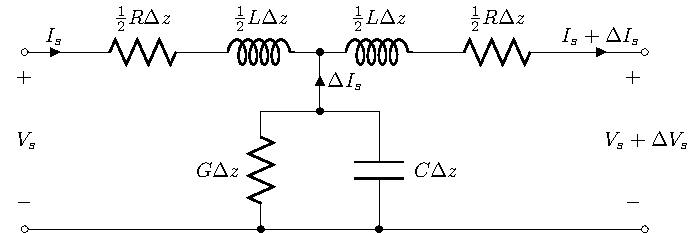
\includegraphics{figTransmissionBaicLines}
\caption{یکساں ترسیلی تار کا چھوٹا حصہ۔ متغیرات $R$، $L$، $C$ اور $G$ تار کی شکل اور مادوں پر منحصر ہیں۔}
\label{شکل_ترسیل_سادہ_نظام}
\end{figure}

یہاں بھی ہم موج کی حرکت \عددیء{\az} جانب تصور کرتے ہیں۔یوں تار کے چھوٹی لمبائی \عددیء{\Delta z} کی مزاحمت \عددیء{R \Delta z}، امالہ \عددیء{L \Delta z}، کپیسٹنس \عددیء{C \Delta z} اور ایصالیت \عددیء{G \Delta z} ہوں گے۔شکل \حوالہ{شکل_ترسیل_سادہ_نظام} میں ترسیلی تار کے اس چھوٹے لمبائی کو دکھایا گیا ہے۔چونکہ تار کا یہ چھوٹا ٹکڑا دونوں اطراف سے بالکل ایک جیسے معلوم ہوتا ہے  لہٰذا اس کے سلسلہ وار اجزاء کو آدھے آدھے ٹکڑوں میں کرتے ہوئے متوازی اجزاء کے دونوں طرف دکھایا گیا ہے۔ہم متوازی اجزاء کو دو برابر ٹکڑون میں کرتے ہوئے سلسلہ وار اجزاء کے دونوں جانب بھی جوڑ سکتے تھے۔

ہم فرض کرتے ہیں کہ شکل \حوالہ{شکل_ترسیل_سادہ_نظام} میں بائیں طرف برقی دباو
\begin{align*}
V=V_0 \cos (\omega t -\beta z +\psi)
\end{align*}
پائی جاتی ہے۔یہ حرکت کرتے موج کی عمومی مساوات ہے۔یولر\فرہنگ{یولر مماثل}\فرہنگ{Euler's identity} مماثل استعمال کرتے ہوئے اس مساوات کو
\begin{align*}
V=\left[ V_0 e^{j(\omega t -\beta z +\psi)}\right]_{\text{حقیقی}}
\end{align*}
لکھا جا سکتا ہے۔اس مساوات میں \عددیء{e^{j\omega t}} اور زیر نوشت میں \عددیء{_\text{حقیق}} کو پوشیدہ رکھتے ہوئے دوری سمتیہ کی صورت میں یوں لکھا جا سکتا ہے
\begin{align*}
V_s =V_0 e^{j \psi} e^{-\beta z}
\end{align*}
جہاں مساوات کے بائیں ہاتھ \عددیء{V_s} لکھتے ہوئے زیرنوشت میں \عددیء{s} یاد دلاتی ہے کہ یہ مساوات دوری سمتیہ کی شکل میں ہے۔ 

شکل \حوالہ{شکل_ترسیل_سادہ_نظام} کے گرد گھومتے ہوئے کرچاف کے برقی دباو کے قانون سے
\begin{align*}
V_s=\left(\frac{R\Delta z}{2} + j \frac{\omega L \Delta z}{2}\right) I_s+\left(\frac{R\Delta z}{2} + j \frac{\omega L \Delta z}{2}\right) \left(I_s+\Delta I_s \right)+V_s+\Delta V_s
\end{align*}
یا
\begin{align*}
\frac{\Delta V_s}{\Delta z} =-\left(R+j\omega L \right) I_s-\frac{1}{2}\left(R+j\omega L \right)\Delta I_s
\end{align*}
لکھا جا سکتا ہے۔اگر \عددیء{\Delta z} کو صفر کے قریب تر کیا جائے تب \عددیء{\Delta I_s} بھی صفر کے قریب تر ہو گا۔یوں \عددیء{\Delta z \to 0 } کی صورت میں اس مساوات کے آخری جزو کو نظر انداز کیا جا سکتا ہے۔یوں اسے
\begin{align}\label{مساوات_ترسیل_دباو_تفرقی_مساوات}
\frac{\dif V_s}{\dif z}=-\left(R+j\omega L \right) I_s
\end{align}
لکھا جا سکتا ہے۔

متوازی اجزاء پر برقی دباو
\begin{align*}
V_s-\left(\frac{R \Delta z}{2}+j\frac{\omega L \Delta z}{2} \right) I_s
\end{align*}
ہے جسے استعمال کرتے ہوئے شکل کو دیکھ کر متوازی اجزاء میں تفرقی رو کے لئے
\begin{align*}
-\Delta I_s = \left[V_s-\left(\frac{R \Delta z}{2}+j\frac{\omega L \Delta z}{2} \right) I_s \right] \left(G \Delta z+j \omega C \Delta z \right)
\end{align*}
یا
\begin{align*}
\frac{\Delta I_s}{\Delta z}=-\left(G+j \omega C \right) V_s +\frac{1}{2}\left(R+j \omega L \right)\left(G+j \omega C \right) I_s \Delta z
\end{align*}
لکھا جا سکتا ہے۔ اگر \عددیء{\Delta z \to 0} کیا جائے تب اس مساوات کے آخری جزو کو نظر انداز کیا جا سکتا ہے اور یوں
\begin{align}\label{مساوات_ترسیل_رو_تفرقی_مساوات}
\frac{\dif I_s}{\dif z}=-\left(G+j \omega C \right) V_s
\end{align}
 حاصل ہوتا ہے۔

یہاں رک کر ذرہ برقی و مقناطیسی امواج کے مساوات کو دوبارہ پیش کرتے ہیں۔میکس ویل کی مساوات
\begin{align*}
\nabla \times \kvec{E}_s=-j \omega \mu \kvec{H}_s
\end{align*}
میں \عددیء{\kvec{E}_s=E_{xs}\ax} اور \عددیء{\kvec{H}_{ys}=H_{ys}\ay}  پر کرنے سے
\begin{align}\label{مساوات_ترسیل_برقی_شدت_تفرقی_مساوات}
\frac{\dif E_{xs}}{\dif z}=-j \omega \mu H_{ys}
\end{align}
ملتا ہے اور اسی طرح
\begin{align*}
\nabla \times \kvec{H}_s=\left(\sigma+j\omega \epsilon \right)\kvec{E}_s
\end{align*}
سے
\begin{align}\label{مساوات_ترسیل_مقناطیسی_شدت_تفرقی_مساوات}
\frac{\dif H_{ys}}{\dif z}=-\left(\sigma+j \omega \epsilon \right) E_{xs}
\end{align}
ملتا ہے۔

مساوات \حوالہ{مساوات_ترسیل_رو_تفرقی_مساوات} کا مساوات \حوالہ{مساوات_ترسیل_مقناطیسی_شدت_تفرقی_مساوات} کے ساتھ موازنا کریں۔غور کرنے سے معلوم ہوتا ہے کہ پہلے مساوات میں \عددیء{I_s} کی جگہ \عددیء{H_{ys}} لکھنے اور اسی طرح \عددیء{G} کی جگہ \عددیء{\sigma}، \عددیء{C} کی جگہ \عددیء{\epsilon} اور \عددیء{V_s} کی جگہ \عددیء{E_{xs}} لکھتے ہوئے دوسری مساوات حاصل کی جا سکتی ہے۔دونوں مساوات بہت قریبی مشابہت رکھتے ہیں۔

اسی طرح مساوات \حوالہ{مساوات_ترسیل_دباو_تفرقی_مساوات} اور مساوات \حوالہ{مساوات_ترسیل_برقی_شدت_تفرقی_مساوات} کو دیکھتے ہوئے  یہی جوڑے یہاں بھی پائے جاتے ہیں، البتہ یہاں \عددیء{L} اور \عددیء{\mu} کی جوڑی بھی پائی جاتی ہے۔ہاں ظاہری طور پر \عددیء{R} کی جوڑی موجود نہیں ہے۔یوں ہم \عددیء{j \omega \mu} کی جوڑی \عددیء{R+j\omega L} لے سکتے ہیں۔

لامحدود یکساں مستوی امواج اور لامحدود لمبائی کی یکساں ترسیلی تار کے سرحدی شرائط ایک جیسے ہیں۔دونوں میں سرحد پایا ہی نہیں جاتا لہٰذا  ہم گزشتہ باب میں حاصل حل
\begin{align*}
E_{xs}=E_{x0} e^{- \gamma z}
\end{align*}
کی طرز پر اب
\begin{align}
V_s=V_0 e^{- \gamma z}
\end{align}
بطور ترسیلی تار کے مساوات کا حل لکھ سکتے ہیں۔یہ برقی دباو کے موج\فرہنگ{موج!برقی دباو}\فرہنگ{wave!voltage} کی مساوات ہے۔یہ موج مثبت \عددیء{z} جانب حرکت کر رہی ہے اور \عددیء{z=0} پر اس کا حیطہ \عددیء{V_0} ہے۔حرکی مستقل\فرہنگ{حرکی مستقل}\فرہنگ{propagation constant}
\begin{align*}
\gamma=\sqrt{j \omega \mu (\sigma +j\omega \epsilon)}
\end{align*}
اب
\begin{align}
\gamma=\alpha+j\beta=\sqrt{(R+j\omega L)(G+j\omega C)}
\end{align}
ہو جائے گا۔طول موج\فرہنگ{طول موج}\فرہنگ{موج!طول}\فرہنگ{wavelength} اب بھی
\begin{align}
\lambda=\frac{2\pi}{\beta}
\end{align}
ہو گا۔موج کی رفتار\فرہنگ{موج!رفتار}\فرہنگ{رفتار!موج}\فرہنگ{phase velocity} اب بھی
\begin{align}
v=\frac{\omega}{\beta}
\end{align}
ہے۔

کامل ترسیلی تار طاقت ضائع نہیں کرتا۔ایسی تار کے مستقل \عددیء{R=G=0} ہوتے ہیں لہٰذا
\begin{align*}
\gamma=j \beta=j \omega \sqrt{LC}
\end{align*}
اور 
\begin{align}
v=\frac{1}{\sqrt{LC}}
\end{align}
ہوں گے۔

اسی طرح مقناطیسی موج
\begin{align*}
H_{ys}=\frac{E_{x0}}{\eta} e^{-\gamma z}
\end{align*}
سے
\begin{align}
I_s=\frac{V_0}{Z_0} e^{-\gamma z}
\end{align}
لکھا جا سکتا ہے جہاں ترسیلی تار کی قدرتی رکاوٹ\فرہنگ{قدرتی رکاوٹ}\فرہنگ{intrinsic impedance} \عددیء{Z_0} کو
\begin{align*}
\eta=\sqrt{\frac{j\omega \mu}{\sigma +j\omega \epsilon}}
\end{align*}
سے
\begin{align}
Z_0=\sqrt{\frac{R+j\omega L}{G+j \omega C}}
\end{align}
لکھا جا سکتا ہے۔

خطہ-1 میں آمدی موج جب خطہ-2 کے سرحد سے ٹکراتی ہے تو اس کا کچھ حصہ بطور انعکاسی موج خطہ-1 میں واپس ہو جاتی ہے۔اس انعکاسی موج اور آمدی موج کی شرح کو شرح انعکاس\فرہنگ{شرح!انعکاس}\فرہنگ{reflection coefficient}
\begin{align*}
\Gamma=\frac{E_{x0}^-}{E_{x0}^+}=\frac{\eta_2-\eta_1}{\eta_2+\eta_1}
\end{align*}
کہتے ہیں۔اسی طرح اگر \عددیء{Z_{01}} قدرتی رکاوٹ کی ترسیلی تار پر آمد موج \عددیء{Z_{02}} قدرتی رکاوٹ کی ترسیلی تار میں داخل ہونا چاہے تو ان کے سرحد سے انعکاسی موج واپس ہو گی۔ایسی انعکاسی موج اور آمدی موج کی شرح
\begin{align}
\Gamma=\frac{V_0^-}{V_0^+}=\frac{Z_{02}-Z_{01}}{Z_{02}+Z_{01}}
\end{align}
 ہو گی۔انعکاسی شرح جانتے ہوئے شرح ساکن موج\فرہنگ{شرح!ساکن موج}\فرہنگ{standing wave ratio}
\begin{align}
s=\frac{1+\abs{\Gamma}}{1-\abs{\Gamma}}
\end{align}
لکھی جا سکتی ہے۔آخر میں اگر \عددیء{z>0} پر \عددیء{\eta=\eta_2} ہو تب \عددیء{z=-l} پر \عددیء{E_{xs}} اور \عددیء{H_{ys}} کی شرح 
\begin{align*}
\eta_{\text{داخلی}}=\eta_1 \frac{\eta_2+j \eta_1 \tan \beta_1 l}{\eta_1 +j \eta_2 \tan \beta_1 l}
\end{align*}
کو داخلی قدرتی رکاوٹ  کہتے ہیں۔اس سے \عددیء{z>0} پر \عددیء{Z_{02}} کی صورت میں ترسیلی تار کے لئے \عددیء{z=-l} پر \عددیء{V_s} اور \عددیء{I_s} کی شرح، یعنی اس کی داخلی قدرتی رکاوٹ\فرہنگ{داخلی قدرتی رکاوٹ}\فرہنگ{رکاوٹ!داخلی قدرتی}\فرہنگ{input intrinsic impedance} کو
\begin{align}
Z_{\text{داخلی}}=Z_{01} \frac{Z_{02}+j Z_{01}\tan \beta_1 l}{Z_{01}+j Z_{02}\tan \beta_1 l}
\end{align}
لکھا جا سکتا ہے۔

%============================
\ابتدا{مشق}
ایک ترسیلی تار جو \عددیء{\omega=\SI{5e8}{\radian\per \second}} پر کام کرتی ہے  کے مستقل \عددیء{R=\SI{0.15}{\ohm\per\meter}}، \عددیء{L=\SI{0.25}{\micro\henry\per\meter}}، \عددیء{G=\SI{8}{\micro\siemens\per\meter}} اور \عددیء{C=\SI{80}{\pico\farad\per\meter}} ہیں۔ اس کے \عددیء{\alpha}، \عددیء{\beta}، \عددیء{\lambda}، \عددیء{v} اور \عددیء{Z_0} حاصل کریں۔

جوابات: \عددیء{\SI{1.57}{\neper\per\meter}}، \عددیء{\SI{2.236}{\radian\per\meter}}، \عددیء{\SI{2.81}{\meter}}، \عددیء{\SI{2.23e8}{\meter\per\second}} اور \عددیء{55.9\phase{-0.029^\circ}\, \ohm}
\انتہا{مشق}
%========================

\حصہ{ترسیلی تار کے مستقل}
اس حصے میں مختلف اشکال کے ترسیلی تار کے مستقل یکجا کرتے ہیں۔ان میں سے عموماً مستقل کو ہم پہلے حاصل کر چکے ہیں، بس انہیں ایک جگہ لکھنا باقی ہو گا۔سب سے پہلے ہم محوری تار کے مستقل اکھٹے کرتے ہیں۔

\begin{figure}
\centering
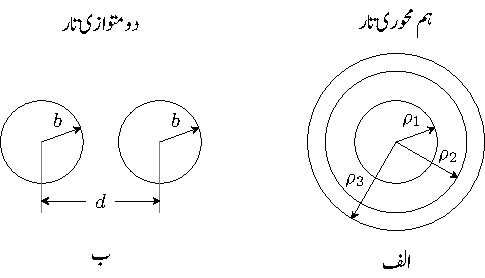
\includegraphics{figTransmissionDifferentLines}
\caption{ہم محوری ترسیلی تار اور دو متوازی ترسیلی تار۔}
\label{شکل_ترسیل_مختلف_ترسیلی_تار}
\end{figure}
\جزوحصہ{ہم محوری تار کے مستقل}
شکل \حوالہ{شکل_ترسیل_مختلف_ترسیلی_تار}-الف میں ہم محوری تار دکھائی گئی ہے جس میں اندرونی تار کا رداس \عددیء{\rho_1} ہے۔بیرونی تار کا اندرونی رداس \عددیء{\rho_2} اور اس کا بیرونی رداس \عددیء{\rho_3} ہیں۔تاروں کے درمیان ذو برق کے مستقل \عددیء{\epsilon}،  \عددیء{\mu} اور \عددیء{\sigma} ہیں۔ صفحہ \حوالہصفحہ{مساوات_کپیسٹر_کپیسٹر_ہم_محوری_تار} پر مساوات میں تار کی لمبائی \عددیء{L=\SI{1}{\meter}} پر کرنے سے اس کی فی میٹر کپیسٹنس
 \begin{align}
C=\frac{Q}{V}=\frac{2\pi\epsilon }{\ln \frac{\rho_2}{\rho_1}}
\end{align}
حاصل ہوتی ہے جبکہ فی میٹر امالہ صفحہ \حوالہصفحہ{مساوات_امالہ_ہم_محوری_کم_تعددی_امالہ} پر مساوات \حوالہ{مساوات_امالہ_ہم_محوری_کم_تعددی_امالہ} دیتا ہے۔
\begin{align}
L_{\text{بیرونی}}=\frac{\mu  I }{2\pi} \ln \frac{\rho_2}{\rho_1}
\end{align}
یہ تار کی بیرونی امالہ ہے۔بلند تعدد پر تار میں برقی رو صرف گہرائی جلد تک محدود رہتی ہے لہٰذا ایسی صورت میں تار کے اندر نہایت کم مقناطیسی بہاو پایا جاتا ہے اور یوں اس کی  اندرونی امالہ قابل نظرانداز ہوتی ہے۔کسی بھی ترسیلی تار کے لئے
\begin{align}\label{مساوات_ترسیلی_امالہ_کپیسٹنس_عمومی_تعلق}
L_{\text{بیرونی}} C=\mu \epsilon
\end{align}
درست ثابت ہوتا ہے۔یوں دونوں ہم محوری تاروں کے درمیان  میں بھری ذو برق کا \عددیء{\epsilon} اور فی میٹر تار کی کپیسٹنس جانتے ہوئے اندرونی امالہ اس مساوات سے حاصل کی جا سکتی ہے۔

کم تعدد پر تار کی اندرونی امالہ کو نظرانداز نہیں کیا جا سکتا۔ایسی صورت میں مساوات \حوالہ{مساوات_امالہ_ہم_محوری_کم_تعددی_فی_میٹر_کل_امالہ}
\begin{align}\label{مساوات_ترسیلی_کم_تعددی_امالہ}
L=\frac{\mu  I }{2\pi} \ln \frac{\rho_2}{\rho_1}+\frac{\mu }{8\pi}+\frac{\mu}{2\pi \left(\rho_3^2-\rho_2^2\right)^2}\left(\rho_3^4 \ln \frac{\rho_3}{\rho_2}-\frac{\rho_2^4}{4}-\frac{3\rho_3^4}{4}+\rho_2^2 \rho_3^2\right)
\end{align}
میں دی گئی فی میٹر تار کی امالہ استعمال کی جائے گی۔یاد رہے کہ یہ امالہ حاصل کرتے ہوئے فرض کیا گیا تھا کہ برقی رو یکساں موصل تار میں گزرتی ہے۔اب ہم جانتے ہیں کہ بلند تعدد پر رو صرف گہرائی جلد تک محدود رہتی ہے لہٰذا کم تعدد پر ہی اس امالہ کو استعمال کیا جا سکتا ہے۔

آئیں ایسی تعدد پر بھی صورت حال دیکھیں جب اندرونی امالہ کی قیمت قابل نظرانداز نہ ہو لیکن گہرائی جلد کے اثر کو بھی نظرانداز نہیں کیا جا سکتا۔ گہرائی جلد کے اثر کی وجہ سے مساوات \حوالہ{مساوات_ترسیلی_کم_تعددی_امالہ} قابل قبول نہیں ہو گی۔اب فرض کرتے ہیں کہ گہرائی جلد \عددیء{\delta} اندرونی تار کے رداس \عددیء{\rho_1} سے بہت کم ہے۔یوں اندرونی تار کے بیرونی باریک تہہ میں برقی رو پائی جائے گی۔برقی رو \عددیء{\az} سمت میں ہے اور چونکہ \عددیء{\kvec{J}_s=\sigma_c \kvec{E}_s} ہوتا ہے لہٰذا تار کی سطح پر \عددیء{\kvec{E}_s} کا مماثل جزو بھی \عددیء{\ax} سمت میں ہو گا۔موصل تار کی موصلیت کو یہاں \عددیء{\sigma_c} لکھا گیا ہے۔ مقناطیسی میدان کی شدت تار کی سطح پر 
\begin{align}\label{مساوات_ترسیلی_ہم_محوری_تار_اندرونی_تار_مقناطیسی_میدان}
H_{\phi s}=\frac{I_s}{2\pi \rho_1}
\end{align}
ہو گی۔اب تار کی سطح پر \عددیء{E_{zs}} اور \عددیء{H_{ys}} کی شرح، مستوی برقی و مقناطیسی موج کی  قدرتی رکاوٹ ہو گی۔اگرچہ ہم نلکی اشکال کی بات کر رہے ہیں لیکن \عددیء{\delta \ll \rho_1} کی بنا پر برقی رو گزارتے باریک تہہ کو \عددیء{\delta} موٹائی اور \عددیء{2\pi \rho_1} چوڑائی کا موصل تصور کیا جا سکتا ہے۔یوں صفحہ \حوالہصفحہ{مساوات_موج_قدرتی_رکاوٹ_موصل_گہرائی_جلد_کے_ساتھ} پر مساوات \حوالہ{مساوات_موج_قدرتی_رکاوٹ_موصل_گہرائی_جلد_کے_ساتھ} سے
\begin{align*}
\left. \right|_{\rho_1}\frac{E_{zs}}{H_{ys}}=\frac{1+j}{\sigma_c \delta}
\end{align*}
لکھا جا سکتا ہے جس میں مساوات \حوالہ{مساوات_ترسیلی_ہم_محوری_تار_اندرونی_تار_مقناطیسی_میدان} پر کرنے سے
\begin{align*}
\left. \frac{E_{zs}}{I_s} \right|_{\rho_1} =\frac{1+j}{2\pi \rho_1 \delta \sigma_c }
\end{align*}
لکھا جا سکتا ہے۔چونکہ \عددیء{E_{zs}} دراصل فی میٹر برقی دباو ہے لہٰذا مندرجہ بالا شرح فی میٹر قدرتی رکاوٹ
\begin{align}\label{مساوات_ترسیلی_رکاوٹ_بلند_تعدد_ہم_محوری}
Z=\left. \frac{E_{zs}}{I_s} \right|_{\rho_1}=R+j \omega L=\frac{1}{2\pi \rho_1 \delta \sigma_c }+j \frac{1}{2\pi \rho_1 \delta \sigma_c }
\end{align}
 کے برابر ہے۔یہ امالہ تار کی اندرونی امالہ ہے جو تار کے موصلیت \عددیء{\sigma_c} پر منحصر ہے۔آپ دیکھ سکتے ہیں کہ کامل موصل کی صورت میں قدرتی رکاوٹ صفر ہو گی۔یوں اندرونی تار کی اندرونی امالہ
\begin{align*}
L_{\rho_1,\text{اندرونی}}=\frac{1}{2\pi \rho_1 \delta \sigma_c \omega}
\end{align*}
ہو گی۔صفحہ \حوالہصفحہ{مساوات_موج_گہرائی_جلد_تعریف} پر مساوات \حوالہ{مساوات_موج_گہرائی_جلد_تعریف} کو \عددیء{\sigma_c=\tfrac{1}{\pi f \mu \delta^2}} لکھتے ہوئے اس میں پر کرنے سے
\begin{align}
L_{\rho_1,\text{اندرونی}}=\frac{\mu \delta}{4 \pi \rho_1} \quad (\delta \ll \rho_1)
\end{align}
حاصل ہوتا ہے۔اسی طریقہ کار سے بیرونی تار کے لئے
\begin{align}
L_{\rho_2,\text{اندرونی}}=\frac{\mu \delta}{4 \pi \rho_2} \quad (\delta \ll \rho_3-\rho_2)
\end{align}
لکھا جا سکتا ہے۔یوں بلند تعدد پر ہم محوری تار کی کل امالہ
\begin{align}
L_{\text{\RL{بلند تعدد}}}=\frac{\mu }{2 \pi }   \left[\ln \frac{\rho_2}{\rho_1} +\frac{\sigma_c}{2} \left(\frac{1}{\rho_1}+\frac{1}{\rho_2} \right)\right] \quad (\delta \ll \rho_1, \, \delta \ll \rho_3-\rho_2)
\end{align}
ہو گا۔مساوات \حوالہ{مساوات_ترسیلی_رکاوٹ_بلند_تعدد_ہم_محوری} بلند تعدد پر قدرتی رکاوٹ کا مزاحمتی حصہ یعنی فی میٹر مزاحمت بھی دیتا ہے جس سے  اندرونی اور بیرونی تاروں کا سلسلہ وار مجموعہ
\begin{align}
R=\frac{1}{2\pi \delta \sigma_c} \left(\frac{1}{\rho_1}+\frac{1}{\rho_2} \right) \quad (\delta \ll \rho_1, \,  \delta \ll \rho_3-\rho_2)
\end{align}
لکھا جا سکتا ہے۔اس مزاحمت کے ساتھ شعاعی اخراج سے پیدا مزاحمتی جزو بھی شامل کیا جا سکتا ہے۔\اصطلاح{بے پناہی}\فرہنگ{بے پناہی}\فرہنگ{پناہ!بے پناہ}\حاشیہب{unshielded}\فرہنگ{unshielded} تار یا ہم محوری تار کے کھلے سر سے شعاعی اخراج ہوتا ہے۔ 

ایسی تعدد جس پر گہرائی جلد کی قیمت رداس سے بہت کم نہ ہو حل کرتے ہوئے \عددیء{بیسل تفاعل}\فرہنگ{بیسل تفاعل}\حاشیہب{Bessel functions}\فرہنگ{Bessel functions} استعمال ہوتے ہیں۔یہاں انہیں حل نہیں کیا جائے گا۔

قدرتی رکاوٹ کو عموماً بیرونی امالہ اور کپیسٹنس  کی صورت میں
\begin{align}
Z_0=\sqrt{\frac{L_{\text{بیرونی}}}{C}} =\frac{1}{2\pi} \sqrt{\frac{\mu}{\epsilon}} \ln \frac{\rho_2}{\rho_1}
\end{align}
لکھا جاتا ہے۔ 

اندرونی اور بیرونی تار کے مابین ذو برق میں سے گزرتی یک سمتی برقی رو \عددیء{I=G V} سے حاصل ہوتی ہے۔اندرونی تار پر \عددیء{\rho_L} اور بیرونی تار پر \عددیء{-\rho_L} کثافت لکیری چارج تصور کرتے ہوئے تاروں کے مابین برقی دباو صفحہ \حوالہصفحہ{مساوات_توانائی_ہم_محوری_تار_برقی_دباو} پر مساوات \حوالہ{مساوات_توانائی_ہم_محوری_تار_برقی_دباو}
\begin{align*}
V=\frac{\rho_L}{2\pi \epsilon} \ln \frac{\rho_2}{\rho_1}
\end{align*}
دیتی ہے۔تاروں کے درمیان ذو برق میں میدان مساوات \حوالہ{مساوات_توانائی_ہم_محوری_تار_ذوبرق_میدان}
\begin{align*}
E_{\rho}=\frac{\rho_L}{2\pi \epsilon \rho}
\end{align*}
دیتی ہے۔ ذو برق کی موصلیت \عددیء{\sigma} لکھتے ہوئے، صفحہ \حوالہصفحہ{مساوات_کپیسٹر-اوہم_قانون_نقطہ_شکل} پر اوہم کے قانون کی نقطہ شکل یعنی مساوات \حوالہ{مساوات_کپیسٹر-اوہم_قانون_نقطہ_شکل} کی مدد سے یوں رداس \عددیء{\rho} پر کثافت  برقی رو
\begin{align*}
J_{\rho}=\sigma E_{\rho}=\frac{\sigma \rho_L}{2\pi \epsilon \rho}
\end{align*}
لکھی جائے گی۔اندرونی تار کے گرد رداس \عددیء{\rho} پر \عددیء{L} لمبائی کی نلکی سطح کا رقبہ \عددیء{2\pi \rho L} ہو گا۔ایسی اکائی لمبائی کی سطح کے رقبہ 
\عددیء{2\pi \rho }  سے کل
\begin{align*}
I= J_{\rho} 2\pi \rho=\frac{\sigma \rho_L}{\epsilon}
\end{align*}
برقی رو گزرے گی۔یوں
\begin{align}
G=\frac{I}{V}=\frac{2\pi \sigma}{\ln \frac{\rho_2}{\rho_1}}
\end{align}
حاصل ہوتا ہے۔

یہاں \عددیء{G} کی قیمت \عددیء{C} کے قیمت سے حاصل کرنا دیکھاتے ہیں۔ایک تار سے دوسرے تار تک \عددیء{\kvec{E}} کی لکیری تکمل سے برقی دباو \عددیء{V} حاصل ہوتا ہے۔صفحہ \حوالہصفحہ{مساوات_کپیسٹر_عمودی_میدان_برابر_کثافت_چارج} پر مساوات \حوالہ{مساوات_کپیسٹر_عمودی_میدان_برابر_کثافت_چارج} کے تحت کسی بھی موصل پر سطحی کثافت چارج، سطح کے عمودی برقی بہاو کے برابر ہوتی ہے، یعنی \عددیء{\rho_S=D_{\text{عمودی}}}۔یوں تار پر کل چارج
\begin{align*}
Q=\int_S \rho_S \dif S = \epsilon \int_S E_{\text{عمودی}} \dif S
\end{align*}
لکھی جا سکتی ہے جہاں \عددیء{S} تار کا سطحی رقبہ ہے اور \عددیء{D=\epsilon E} لکھا گیا گا۔یوں
\begin{align}\label{مساوات_ترسیلی_ہم_محوری_تار_کپیسٹنس_عمومی_مساوات}
C=\frac{Q}{V}=\frac{\epsilon \int_S E_{\text{عمودی}} \dif S}{V}
\end{align}
ہو گا۔اب موصل کے سطح پر \عددیء{E_{\text{عمودی}}} جانتے ہوئے یہاں کثافت برقی رو \عددیء{J=\sigma E_{\text{عمودی}}} لکھی جا سکتی ہے لہٰذا تار کے سطح سے خارج کل برقی رو
\begin{align*}
I=\sigma \int_S E_{\text{عمودی}} \dif S
\end{align*}
ہو گی۔یوں دو تاروں کے مابین ایصالیت
\begin{align}\label{مساوات_ترسیلی_ہم_محوری_تار_ایصالیت_عمومی_مساوات}
G=\frac{I}{V}=\frac{\sigma \int_S E_{\text{عمودی}} \dif S}{V}
\end{align}
ہو گی۔مساوات \حوالہ{مساوات_ترسیلی_ہم_محوری_تار_کپیسٹنس_عمومی_مساوات} اور مساوات \حوالہ{مساوات_ترسیلی_ہم_محوری_تار_ایصالیت_عمومی_مساوات} کو دیکھ کر
\begin{align}\label{مساوات_ترسیلی_کپیسٹنس_ایصالیت_تعلق}
G=\frac{\sigma}{\epsilon} C
\end{align}
لکھا جا سکتا ہے جو کسی بھی ترسیلی تار کے لئے درست ہے
%=====================
\ابتدا{مشق}
ایک ہم محوری تار جس کے \عددیء{\rho_1=\SI{1}{\milli\meter}}،  \عددیء{\rho_2=\SI{3.49}{\milli \meter}} اور \عددیء{\sigma_c=\SI{3.82e7}{\siemens\per\meter}} ہیں کے ذو برق کے مستقل \عددیء{\mu_R=1}، \عددیء{\epsilon_R=2.25} اور \عددیء{\sigma=\SI{10}{\micro \siemens \per \meter}} ہیں۔ اس کا فی میٹر کپیسٹنس، بیرونی اور اندرونی امالہ حاصل کریں۔ترسیلی تار کے \عددیء{\alpha}، \عددیء{\beta} اور \عددیء{Z_0} بھی حاصل کریں۔

جوابات: \عددیء{\SI{0.1}{\nano\farad\per\meter}}، \عددیء{\SI{0.25}{\micro\henry\per\meter}}، \عددیء{\SI{1.29}{\nano\henry\per\meter}}،  \عددیء{\SI{0.014}{\neper\per\meter}}، \عددیء{\SI{15.1}{\radian\per\meter}} اور
  \عددیء{50\phase{0.055^\circ} \, \si{\ohm}}
\انتہا{مشق}
%====================
\جزوحصہ{دو متوازی تار کے مستقل}
شکل \حوالہ{شکل_ترسیل_مختلف_ترسیلی_تار}-ب میں دو متوازی ترسیلی تار دکھائی گئی ہے۔تار کا رداس \عددیء{b}، تاروں کے مابین فاصلہ \عددیء{d} جبکہ تار کی موصلیت \عددیء{\sigma_c} ہے۔تاروں کے گرد ذو برق کے مستقل \عددیء{\epsilon}،  \عددیء{\mu} اور \عددیء{\sigma} ہیں۔ اس تار کی کپیسٹنس صفحہ \حوالہصفحہ{مساوات_کپیسٹر_نلکی_زمین_کپیسٹنس} پر مساوات \حوالہ{مساوات_کپیسٹر_نلکی_زمین_کپیسٹنس} کی نصف ہو گی۔اس کی وجہ وہیں پر مساوات کے نیچے سمجھائی گئی ہے۔یوں فی میٹر تار کی کپیسٹنس
\begin{align}
C=\frac{\pi\epsilon }{\cosh^{-1} \frac{d}{2 b}}
\end{align}
ہو گی۔اگر \عددیء{b\ll d} ہو تب مساوات \حوالہ{مساوات_کپیسٹر_نلکی_زمین_کپیسٹنس_ب} سے
\begin{align*}
C=\frac{\pi\epsilon }{ \ln \frac{d}{b}} \quad( b \ll d )
\end{align*}
لکھا جا سکتا ہے۔مساوات \حوالہ{مساوات_ترسیلی_امالہ_کپیسٹنس_عمومی_تعلق} سے تار کی فی میٹر بیرونی امالہ
\begin{align*}
L_{\text{بیرونی}}=\frac{\mu}{\pi} \cosh^{-1} \frac{d}{2b}
\end{align*}
یا
\begin{align*}
L_{\text{بیرونی}}=\frac{\mu}{\pi} \ln \frac{d}{b} \quad(b \ll d)
\end{align*}
لکھی جا سکتی ہے جبکہ بلند تعدد پر فی میٹر کل امالہ
\begin{align}
L_{\text{\RL{بلند تعدد}}}=\frac{\mu}{\pi} \left(\frac{\delta}{2b}+\cosh^{-1} \frac{d}{2 b} \right) \quad(\delta \ll b)
\end{align}
ہے۔تار کی بیرونی \عددیء{\delta} تہہ برقی رو گزارتی ہے۔اس تہہ کا رقبہ عمودی تراش \عددیء{S=2\pi b \delta} ہے لہٰذا فی میٹر مزاحمت
\begin{align}
R=\frac{l}{\sigma_c S}=\frac{1}{\pi b \delta \sigma_c}
\end{align}
ہو گی جہاں دونوں تاروں کی مزاحمت سلسلہ وار جڑے ہیں۔مساوات \حوالہ{مساوات_ترسیلی_کپیسٹنس_ایصالیت_تعلق} سے فی میٹر تار کی ایصالیت
\begin{align}
G=\frac{\pi \sigma}{\cosh^{-1} \frac{d}{2b}}
\end{align}
حاصل ہوتی ہے۔

بیرونی امالہ اور کپیسٹنس استعمال کرتے ہوئے قدرتی مزاحمت
\begin{align}
Z_0=\frac{1}{\pi} \sqrt{\frac{\mu}{\epsilon}} \cosh^{-1} \frac{d}{2b}
\end{align}
حاصل ہوتا ہے۔

\begin{figure}
\centering
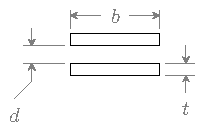
\includegraphics{figTransmissionStripLine}
\caption{سطح مستوی ترسیلی تار۔}
\label{شکل_ترسیلی_سطح_مستوی}
\end{figure}

\جزوحصہ{سطح مستوی ترسیلی تار}
شکل \حوالہ{شکل_ترسیلی_سطح_مستوی} میں \اصطلاح{سطح مستوی ترسیلی تار}\فرہنگ{سطح مستوی ترسیلی تار}\فرہنگ{ترسیلی!سطح مستوی}\حاشیہب{stripline}\فرہنگ{stripline} دکھایا گیا ہے جس میں \عددیء{b} چوڑائی اور \عددیء{t} موٹائی کے دو متوازی موصل چادر دکھائے گئے ہیں جن کے مابین فاصلہ \عددیء{d} ہے۔موصل چادر کی موصلیت \عددیء{\sigma_c} جبکہ ارد گرد کے ذو برق کے مستقل \عددیء{\epsilon}، \عددیء{\mu} اور \عددیء{\sigma} ہیں۔

اگر \عددیء{b\gg d} ہو تب ان چادروں کی فی میٹر کپیسٹنس  
\begin{align}
C=\frac{\epsilon \text{رقبہ}}{ \text{فاصلہ}} = \frac{\epsilon b}{d}
\end{align}
ہو گی۔یوں مساوات \حوالہ{مساوات_ترسیلی_امالہ_کپیسٹنس_عمومی_تعلق} سے فی میٹر بیرونی امالہ
\begin{align}
L_{\text{بیرونی}}=\frac{\mu \epsilon}{C}=\frac{\mu d}{b}
\end{align}
ہو گی۔امید کی جاتی ہے کہ آپ گہرائی جلد استعمال کرتے ہوئے اندرونی امالہ حاصل کر سکتے ہیں۔یوں کل امالہ
\begin{align}
L=\frac{\mu d}{b}+\frac{2}{\sigma_c \delta b w}=\frac{\mu}{b} (d+\delta) \quad (\delta \ll t)
\end{align}
ہو گی جہاں گہرائی جلد کو چادر کی موٹائی سے بہت کم تصور کیا گیا ہے۔

بلند تعدد پر برقی رو چادروں کے آمنے سامنے  سطحوں پر گہرائی جلد تک محدود ہو گی۔یوں برقی رو رقبہ \عددیء{b \delta} سے گزرے گی جس سے ایک تار کے اکائی لمبائی کی مزاحمت \عددیء{\tfrac{1}{\sigma_c b \delta}} حاصل ہوتی ہے۔یوں اکائی لمبی تار کے دونوں حصوں کی سلسلہ وار جڑی کل مزاحمت
\begin{align}
R=\frac{2}{\sigma_c b \delta} \quad (\delta \ll t)
\end{align}
ہو گی۔ 

مساوات \حوالہ{مساوات_ترسیلی_کپیسٹنس_ایصالیت_تعلق} سے
\begin{align}
G=\frac{\sigma b}{d}
\end{align}
لکھی جا سکتی ہے۔

ان معلومات سے سطح مستوی ترسیلی تار کی قدرتی رکاوٹ
\begin{align}
Z_0=\sqrt{\frac{L_{\text{بیرونی}}}{C}}=\sqrt{\frac{\mu}{\epsilon}} \frac{d}{b}
\end{align}
لکھی جا سکتی ہے۔
%=======================
\ابتدا{مشق}
مندرجہ بالا تینوں اقسام کے ترسیلی تار \عددیء{\SI{400}{\mega \hertz}} پر کام کر رہے ہیں۔ان میں طاقت کے ضیاع کو نظرانداز کرتے ہوئے تمام کے لئے \عددیء{\lambda} اور \عددیء{\Gamma} حاصل کریں۔ہم محوری تار کا \عددیء{\rho_1=\SI{0.5}{\milli\meter}}، \عددیء{\rho_2=\SI{2.8}{\milli \meter}}، \عددیء{\mu_R=1} اور \عددیء{\epsilon_R=3.1} ہیں۔ متوازی تار کے \عددیء{b=\SI{0.5}{\milli\meter}}، \عددیء{d=\SI{9}{\milli\meter}}، \عددیء{\mu_R=1} اور \عددیء{\epsilon_R=5} ہیں۔ مستوی سطح کے \عددیء{d=\SI{0.2}{\milli\meter}}، \عددیء{b=\SI{5}{\milli\meter}}، \عددیء{\mu_R=1} اور \عددیء{\epsilon_R=2.2} ہیں۔

جوابات: \عددیء{\SI{42.6}{\centi\meter}}، \عددیء{0.26}، \عددیء{\SI{33.5}{\centi\meter}}، \عددیء{-0.215}، \عددیء{\SI{50.6}{\centi\meter}}، \عددیء{0.816}
\انتہا{مشق}
%=====================

\حصہ{ترسیلی تار کے چند مثال}
اس حصے میں گزشتہ حصوں کے نتائج استعمال کرتے ہوئے چند مثال کرتے ہیں۔یہاں تمام ترسیلی تاروں کو بے ضیاع تار تصور کیا جائے گا۔

شروع دو متوازی ترسیلی تار سے کرتے ہیں جس کی قدرتی رکاوٹ \عددیء{\SI{300}{\ohm}} ہے۔ ایسی تار \اصطلاح{ٹی وی}\فرہنگ{ٹی وی}\حاشیہب{TV, television}\فرہنگ{TV} کے اینٹینا اور ٹی وی کے مابین لگائی جاتی ہے۔شکل \حوالہ{شکل_ترسیلی_اینٹینا_تا_ٹی_وی}-الف میں اس طرح جڑے ترسیلی نظام کو دکھایا گیا ہے۔اینٹینا کا تھونن\فرہنگ{تھونن}\حاشیہب{Thevenin}\فرہنگ{Thevenin} مساوی دور استعمال کیا گیا ہے جو ایک عدد منبع برقی دباو \عددیء{V_s} اور اس کے ساتھ سلسلہ وار  جڑی \عددیء{\SI{300}{\ohm}} کی مزاحمت پر مشتمل ہے۔ترسیلی تار ٹی وی کے برقیاتی دور کے بالکل شروع میں نسب ابتدائی ایمپلی فائر سے جڑتی ہے جس کا داخلی مزاحمت \عددیء{\SI{300}{\ohm}} ہے۔ٹی وی کو اسی مزاحمت سے ظاہر کیا گیا ہے۔اس مثال میں ٹی وی بطور برقی بار کردار ادا کرتا ہے۔ٹی وی اسٹیشن سے خارج \عددیء{\SI{100}{\mega \hertz}} کے برقی و مقناطیسی امواج اس اینٹینا میں \عددیء{\SI{5}{\milli\volt}} کا اشارہ پیدا کرتی ہیں۔ترسیلی تار کے مستقل ایسے ہیں کہ اس میں اشارات کی رفتار \عددیء{\SI{2.5e8}{\meter\per\second}} ہے۔

\begin{figure}
\centering
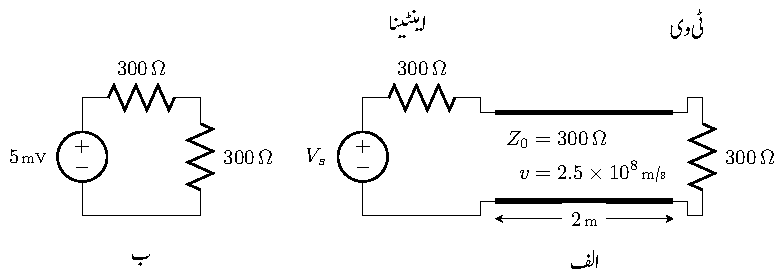
\includegraphics{figTransmissionThreeHundredOhmExample}
\caption{ترسیلی تار اینٹینا کو ٹی وی سے جوڑ رہی ہے۔}
\label{شکل_ترسیلی_اینٹینا_تا_ٹی_وی}
\end{figure}

چونکہ برقی بار کی مزاحمت اور ترسیلی تار کی قدرتی مزاحمت برابر ہیں لہٰذا ترسیلی تار اور برقی بار ہمہ رکاوٹ ہیں۔یوں برقی بار پر انعکاس نہیں پایا جائے گا لہٰذا شرح انعکاس
\begin{align*}
\Gamma=\frac{300-300}{300+300}=0
\end{align*}
 صفر اور شرح ساکن موج
\begin{align*}
s=\frac{1-\abs{\Gamma}}{1+\abs{\Gamma}}=\frac{1-0}{1+0}=1
\end{align*}
ایک کے برابر ہوں گے۔اشارے کے تعدد پر ترسیلی تار میں طول موج
\begin{align*}
\lambda=\frac{v}{f}=\frac{2.5 \times 10^8}{100\times 10^6}=\SI{2.5}{\meter}
\end{align*}
اور زاویائی مستقل
\begin{align*}
\beta=\frac{2\pi}{\lambda}=\frac{2\pi}{2.5}=0.8 \pi\, \si{\radian \per \meter}
\end{align*}
 ہیں۔ترسیلی تار کی برقی لمبائی
\begin{align*}
\beta l =0.8 \pi \times 2=1.6 \pi \, \si{\radian}
\end{align*} 
یا \عددیء{288^\circ} ہے جسے \عددیء{0.8} طول موج بھی کہا جاتا ہے۔ 

شکل \حوالہ{شکل_ترسیلی_اینٹینا_تا_ٹی_وی}-ب میں داخلی جانب کا صورت حال دکھایا گیا ہے۔داخلی جانب چونکہ اینٹینا کی مزاحمت \عددیء{\SI{300}{\ohm}} ہے اور ترسیلی تار کی قدرتی رکاوٹ بھی \عددیء{\SI{300}{\ohm}} ہے لہٰذا  اینٹینا اور ترسیلی تار ہمہ رکاوٹ ہیں۔اینٹینا میں پیدا \عددیء{\SI{5}{\milli \volt}} کا اشارہ ترسیلی تار کے قدرتی رکاوٹ پر 
\begin{align*}
\frac{5 \times 10^{-3} \times 300}{300+300}=\SI{2.5}{\milli \volt}
\end{align*}
پیدا کرے گا۔اینٹینا اور ترسیلی تار ہمہ رکاوٹ ہیں لہٰذا منبع طاقت \عددیء{V_s} ترسیلی تار میں زیادہ سے زیادہ طاقت بھیجے گا۔ترسیلی تار کے داخلی جانب پیدا \عددیء{\SI{2.5}{\milli \volt}} کا اشارہ تار میں سے گزرتے ہوئے برقی بار تک پہنچے گا البتہ یہ داخلی اشارے سے \عددیء{1.6 \pi} ریڈیئن پیچھے ہو گا۔یوں اگر ترسیلی تار کا داخلی اشارہ
\begin{align*}
V_{\text{داخلی}}=2.5 \cos 2\pi 10^8 t \quad \si{\milli \volt}
\end{align*}
ہو تب برقی بار پر اشارہ
\begin{align*}
V_{\text{\RL{بار}}}=2.5 \cos (2\pi 10^8 t-1.6 \pi) \quad \si{\milli \volt}
\end{align*}
ہو گا۔داخلی برقی رو
\begin{align*} 
I_{\text{داخلی}}=\frac{V_{\text{داخلی}}}{300} =8.33 \cos 2\pi 10^8 t \quad \si{\micro \ampere}
\end{align*}
اور برقی بار پر برقی رو
\begin{align*} 
I_{\text{بار}}=\frac{V_{\text{داخلی}}}{300} =8.33 \cos (2\pi 10^8 t -1.6\pi) \quad \si{\micro \ampere}
\end{align*}
ہوں گے۔چونکہ ترسیلی تار بے ضیاع تار ہے لہٰذا جو طاقت اسے داخلی جانب فراہم کی جاتی ہے وہی طاقت خارجی جانب برقی بار کو  مہیا کر دی جاتی ہے۔
\begin{align*}
P_{\text{داخلی}} =P_{\text{بار}}= V_{\text{موثر}} I_{\text{موثر}}=\frac{ 2.5 \times 10^{-3}}{\sqrt{2}} \times \frac{8.33 \times 10^{-6}}{\sqrt{2}}=\SI{10.41}{\nano\watt} 
\end{align*}
مزاحمتی بار کی طاقت کا حساب لگاتے وقت یاد رہے کہ \عددیء{P=VI} میں برقی دباو اور برقی رو کے موثر\فرہنگ{موثر}\حاشیہب{RMS, effective}\فرہنگ{RMS} قیمتیں استعمال کی جاتی ہیں۔سائن نما موج کی موثر قیمت موج کی چوٹی تقسیم \عددیء{\sqrt{2}} کے برابر ہوتی ہے۔

اب پہلے ٹی وی کے متوازی دوسرا ٹی وی نسب کرنے کے اثرات پر غور کرتے ہیں۔دوسرے ٹی وی کا داخلی مزاحمت بھی \عددیء{\SI{300}{\ohm}} ہے۔یوں اب ترسیلی تار کے خارجی جانب کل \عددیء{\SI{150}{\ohm}} کا بار پایا جاتا ہے۔اس طرح شرح انعکاس
\begin{align*}
\Gamma=\frac{150-300}{150=300}=-\frac{1}{3}
\end{align*}
یا
\begin{align}
\Gamma=\frac{1}{3}\phase{\pi}
\end{align}
حاصل ہوتی ہے اور شرح ساکن موج
\begin{align*}
s=\frac{1+\frac{1}{3}}{1-\frac{1}{3}}=2
\end{align*}
ہوں گے۔ترسیلی تار کی داخلی مزاحمت اب \عددیء{\SI{300}{\ohm}} کے بجائے
\begin{align*}
Z_{\text{داخلی}} &=Z_0 \frac{Z_L +j Z_0 \tan \beta l}{Z_0+j Z_L \tan \beta l}=300 \frac{150+j 300 \tan 288^\circ}{300+j 150 \tan 288^\circ}\\
&=509.7 \phase{-23.79^\circ}=466.39-j 205.6 \quad \si{\ohm} 
\end{align*}
ہو گی جو کپیسٹر کی خاصیت رکھتی ہے۔کپیسٹر کی خاصیت کا مطلب یہ ہے کہ ترسیلی تار کے برقی میدان میں مقناطیسی میدان سے زیادہ توانائی ذخیرہ ہے۔داخلی رو
\begin{align*}
I_{s,\text{داخلی}} = \frac{0.005}{300+466.39-j 205.6} =6.3013\phase{15.017^\circ} \quad \si{\micro \ampere}
\end{align*} 
ہے اور یوں ترسیلی تار کو داخلی جانب
\begin{align*}
P_{\text{داخلی}}= \frac{1}{2} \left(6.3013 \times 10^{-6} \right)^2 \times 466.39 = \SI{9.2593}{\nano \watt}
\end{align*}
طاقت فراہم کی جا رہی ہے۔بے ضیاع تار تمام کی تمام طاقت خارجی جانب منتقل کرے گا لہٰذا \عددیء{\SI{150}{\ohm}} کے بار کو \عددیء{\SI{9.2593}{\nano \watt}} حاصل ہو گا جو گزشتہ جواب یعنی \عددیء{\SI{10.41}{\nano\watt} } سے قدر کم ہے۔یہ کمی انعکاس کی وجہ سے پیدا ہوئی۔ کہانی یہاں ختم نہیں ہوتی۔یہ طاقت دونوں ٹی وی میں برابر تقسیم ہو گا لہٰذا ہر ٹی وی کو صرف \عددیء{\SI{4.6297}{\nano\watt} }  طاقت مہیا ہو گا۔چونکہ ایک ٹی وی \عددیء{\SI{300}{\ohm}} مزاحمت رکھتا ہے لہٰذا ٹی وی پر پیدا برقی دباو
\begin{align*}
4.6297 \times 10^{-9} = \frac{\abs{V_{s,\text{\RL{بار}}}}^2}{2 \times 300}
\end{align*}
یعنی
\begin{align*}
\abs{V_{s,\text{\RL{بار}}}}=\SI{1.66667}{\milli \volt}
\end{align*}
ہو گا۔یہ قیمت \عددیء{\SI{2.5}{\milli \volt}} سے بہت کم ہے جو اکیلے ٹی وی پر پیدا ہوتی ہے۔

آئیں ترسیلی تار پر برقی دباو کی چوٹی، نشیب اور ان کے مقامات کے علاوہ دیگر معلومات بھی حاصل کریں۔اگر ہم برقی دباو کے معلومات حاصل کر سکیں تو ظاہر ہے کہ برقی رو کے معلومات بھی حاصل کر پائیں گے۔گزشتہ باب میں مستوی امواج کے لئے یہی معلومات حاصل کی گئیں تھیں۔ وہاں استعمال کئے گئے ترکیب یہاں بھی کارآمد ثابت ہوں گے۔برقی دباو موج کے چوٹی کے مقامات مساوات \حوالہ{مساوات_موج_مقام_بلنتر_دباو}
\begin{align*}
-\beta_1 z_{\text{بلندتر}} =\frac{\phi}{2}+ n \pi \quad (n=0,\mp1,\mp 2, \cdots)
\end{align*}
دیتا ہے۔اس میں \عددیء{\beta=0.8 \pi} اور \عددیء{\phi=\pi} پر کرنے سے
\begin{align*}
z_{\text{بلندتر}} &=\frac{1}{-0.8 \pi} \left(\frac{\pi}{2}+n \pi \right)\\
&=-1.25\left(\frac{1}{2}+n \right)
\end{align*}
حاصل ہوتا ہے جس میں \عددیء{n=0}  اور \عددیء{n=1} پر کرنے سے
\begin{align*}
z_{\text{بلندتر}}=  \SI{-0.625}{\meter}  \quad \text{اور} \quad \SI{-1.875}{\meter}
\end{align*}
حاصل ہوتے ہیں جو درست جوابات ہیں۔اگر \عددیء{n=2} پر کیا جائے تو \عددیء{z_{\text{بلندتر}}=\SI{-3.125}{\meter}} حاصل ہوتا ہے جبکہ تار کی کل لمبائی صرف دو میٹر ہے لہٰذا اس جواب کو رد کیا جاتا ہے۔اسی طرح \عددیء{n=-1} پر کرنے سے  \عددیء{z_{\text{بلندتر}}=\SI{+0.625}{\meter}} حاصل ہوتا ہے جبکہ تار منفی \عددیء{z} محدد پر پائی جاتی ہے لہٰذا اس جواب کو بھی رد کیا جاتا ہے۔

موج کے چوٹی سے \عددیء{\tfrac{\lambda}{4}} فاصلے پر نشیب پائے جاتے ہیں، لہٰذا ان کے مقامات
\begin{align*}
z_{\text{کمتر}} = \SI{0}{\meter} \quad \text{اور} \quad \SI{-1.25}{\meter}
\end{align*}
ہوں گے۔آپ نے دیکھا کہ سرحد پر برقی دباو کا نشیب پایا جاتا ہے۔آپ کو یاد ہو گا کہ حقیقی \عددیء{Z_0} اور \عددیء{Z_L} کی صورت میں اگر \عددیء{Z_0<Z_L} ہو تب سرحد پر موج کا نشیب ہی پایا جاتا ہے۔

چونکہ سرحد پر موج کا نشیب ہے اور ہم جانتے ہیں کہ ٹی وی پر \عددیء{\SI{1.66}{\milli \volt}} ہے لہٰذا دباو کی کمتر قیمت یہی ہے اور \عددیء{s=2} سے دباو کی چوٹی اس کے دگنا یعنی \عددیء{\SI{3.32}{\milli\volt}} حاصل ہوتی ہے۔ترسیلی تار کے داخلی سرے پر برقی دباو
\begin{align*}
V_{s,\text{داخلی}} = I_{s,\text{داخلی}} Z_{\text{داخلی}} =\left(6.3013 \times 10^{-6}\phase{15.017^\circ} \right)\left(509.7 \phase{-23.79^\circ} \right) =0.00321175\phase{-8.77^\circ}
\end{align*}
ہو گی جو تقریباً موج کے چوٹی کے برابر ہے۔ایسا اس لئے ہے کہ سرحد سے \عددیء{\tfrac{\lambda}{4}}  فاصلے پر چوٹی پائی جاتی ہے جس سے ہر \عددیء{0.5\lambda} فاصلے پر چوٹی ہو گی لہٰذا سرحد سے \عددیء{\tfrac{3\lambda}{4}} فاصلے پر بھی چوٹی متوقع ہے جو تار کے داخلی سرے کے بہت قریب نقطہ ہے۔آپ ترسیلی تار کی داخلی برقی دباو یوں
\begin{align*}
V_{s,\text{داخلی}}= \frac{Z_{\text{داخلی}} V_s}{Z_{\text{داخلی}}+300}  = \frac{(466.39-j 205.6) \times 0.005}{466.39-j 205.6+300}=0.00321175\phase{-8.77^\circ}
\end{align*}
 بھی حاصل کر سکتے ہیں۔

آخر میں داخلی برقی دباو اور بار پر برقی دباو کا زاویائی تعلق دیکھتے ہیں۔اگرچہ ہم دونوں برقی دباو کے قیمتیں حاصل کر چکے ہیں، ان کے زاویائی معلومات ابھی  تک نہیں حاصل کی گئیں۔مساوات \حوالہ{مساوات_موج_ساکن_مخلوط_موج} کی مدد سے  تار پر کسی بھی نقطے پر برقی دباو
\begin{align*}
V_{s}=\left(e^{-j\beta z}+\Gamma e^{j\beta z} \right) V_0^+
\end{align*} 
لکھا جا سکتا ہے۔چونکہ ہمیں تار کے داخلی سرے پر دباو معلوم ہے لہٰذا اس میں \عددیء{z=-l} پر کرنے سے
\begin{align*}
V_{s,\text{داخلی}}=\left(e^{j\beta l}+\Gamma e^{-j\beta l} \right) V_0^+
\end{align*} 
حاصل ہوتا ہے جسے \عددیء{V_0^+} کے لئے حل کرتے ہیں
\begin{align*}
V_0^+=\frac{V_{s,\text{داخلی}}}{e^{j\beta l}+\Gamma e^{-j\beta l} }=\frac{0.00321175\phase{-8.77^\circ}}{e^{j1.6\pi}-\frac{1}{3} e^{-j1.6\pi} }=0.0025 \phase{-72^\circ}
\end{align*}
اور یوں بار یعنی \عددیء{z=0} پر برقی دباو اب حاصل کی جا سکتی ہے
\begin{align*}
V_{s,\text{بار}} =\left(1+\Gamma \right) V_0^+=0.001666\phase{-72^\circ}=0.001666\phase{-288^\circ}
\end{align*}
یہاں حاصل جواب کی حتمی قیمت اور کچھ دیر پہلے حاصل کی گئی بار پر برقی دباو کی حتمی قیمت برابر ہیں۔تار کے داخلی سرے پر دباو کا زاویہ \عددیء{-8.77^\circ} جبکہ تار کے خارجی سرے پر دباو کا زاویہ \عددیء{72^\circ} ہے۔یوں ان کے مابین فرق \عددیء{80.77^\circ} یعنی \عددیء{-279.23^\circ} ہے۔انعکاسی موج کی عدم موجودگی میں یہ فرق
 \عددیء{-288^\circ} یعنی تار کی زاویائی لمبائی جتنا ہوتا ہے۔

آخری مثال کے طور پر ہم اس ترسیلی تار کے خارجی سرے پر صرف کپیسٹر \عددیء{Z_L=-j300\, \si{\ohm}} نسب کر کے دیکھتے ہیں۔کپیسٹر میں توانائی ضائع نہیں ہوتی۔یہ حقیقت شرح انعکاس
\begin{align*}
\Gamma=\frac{-j300-300}{-j300+300}=-j=1\phase{-90^\circ}
\end{align*}
 سے صاف ظاہر ہے جو انعکاسی موج کا حیطہ آمدی موج کے برابر دیتا ہے۔شرح ساکن موج یوں
\begin{align*}
s=\frac{1+\abs{-j}}{1-\abs{-j}}=\infty
\end{align*}
ہو گا جس سے موج کا نشیب عین صفر کے برابر حاصل ہوتا ہے۔ترسیلی تار کی داخلی قدرتی رکاوٹ
\begin{align*}
Z_{\text{داخلی}}=300 \frac{-j300+j300 \tan 288^\circ}{300+j(-j300)\tan 288^\circ}=j 589
\end{align*}
ہو گی جو خیالی عدد ہے لہٰذا اسے اوسط طاقت فراہم نہیں کی جا سکتی۔

ترسیلی تار کے مسائل ترسیمی طریقے سے نہایت خوش اسلوبی سے حل ہوتے ہیں۔ان میں \اصطلاح{سمتھ نقشہ}\فرہنگ{سمتھ نقشہ}\فرہنگ{نقشہ!سمتھ}\حاشیہب{Smith chart}\فرہنگ{Smith chart} زیادہ اہم ہے۔اگلے حصے میں اسی پر غور کیا جائے گا۔

\حصہ{ترسیمی تجزیہ، سمتھ نقشہ}
سمتھ نقشہ بنیادی طور پر شرح انعکاس
\begin{align*}
\Gamma=\frac{Z_L-Z_0}{Z_L+Z_0}
\end{align*}
کی مساوات پر منحصر ہے۔اس نقشے میں بار کی بجائے بار تقسیم قدرتی رکاوٹ یعنی \عددیء{\tfrac{Z_L}{Z_0}} استعمال کی جاتی ہے۔اس شرح کو
\begin{align*}
z=r+jx=\frac{Z_L}{Z_0}=\frac{R_L+j X_L}{Z_0}
\end{align*}
لکھا جا سکتا ہے جہاں \عددیء{z} کارتیسی محدد کا متغیرہ نہیں بلکہ اس شرح کو ظاہر کرتی ہے۔یوں
\begin{align*}
\Gamma=\frac{z-1}{z+1}
\end{align*}
  اور
\begin{align*}
z=\frac{1+\Gamma}{1-\Gamma}
\end{align*}
لکھے جا سکتے ہیں۔شرح انعکاس کو حقیقی اور خیالی اجزاء
\begin{align*}
\Gamma=\Gamma_r+j \Gamma_i
\end{align*}
کی صورت میں لکھتے ہوئے
\begin{align*}
r+j x =\frac{1+\Gamma_r+j \Gamma_i}{1-\Gamma_r-j\Gamma_i}
\end{align*} 
کے حقیقی اور خیالی اجزاء علیحدہ کرتے ہوئے
\begin{align}
r&=\frac{1-\Gamma_r^2-\Gamma_i^2}{\left(1-\Gamma_r\right)^2+\Gamma_i^2}\\
x&=\frac{2\Gamma_i}{\left(1-\Gamma_r\right)^2+\Gamma_i^2}
\end{align}
لکھے جا سکتے ہیں جنہیں کچھ الجبرا کے بعد
\begin{align}
\left(\Gamma_r-\frac{r}{1+r}\right)^2+\Gamma_i^2&=\left(\frac{1}{1+r}\right)^2 \label{مساوات_ترسیلی_سمتھ_دائرہ_الف}\\
\left(\Gamma_r-1 \right)^2+\left(\Gamma_i-\frac{1}{x} \right)^2&=\left(\frac{1}{x}\right)^2  \label{مساوات_ترسیلی_سمتھ_دائرہ_ب}
\end{align}
لکھا جا سکتا ہے۔اگر کارتیسی محدد کے متغیرات \عددیء{\Gamma_r} اور \عددیء{\Gamma_i} رکھے جائیں تو مندرجہ بالا دونوں مساوات گول دائروں کے مساوات ہوں گے۔

مساوات \حوالہ{مساوات_ترسیلی_سمتھ_دائرہ_الف} کے دائروں پر پہلے غور کرتے ہیں۔اگر \عددیء{r=0} ہو تب یہ مساوات اکائی رداس کا دائرہ دیتی ہے جس کا درمیانہ نقطہ محدد کے \عددیء{(0,0)} پر ہے۔خیالی برقی بار کی صورت میں شرح انعکاس کی حتمی قیمت ایک ہی ہوتی ہے۔اسی طرح \عددیء{r=\infty} کی صورت میں دائرے کا رداس صفر جبکہ اس کا درمیانہ نقطہ محدد پر \عددیء{(1,0)} ہے۔یوں یہ دائرہ صرف اسی نقطے یعنی \عددیء{\Gamma=1} تک محدود ہے۔اب \عددیء{r=\infty} سے مراد \عددیء{Z_L-\infty} ہے جس سے شرح انعکاس \عددیء{\Gamma=1} ہی حاصل ہوتی ہے۔ایک آخری مثال \عددیء{r=1} کی لیتے ہیں جس سے \عددیء{0.5} رداس کا دائرہ حاصل ہوتا ہے جس کا درمیانہ نقطہ \عددیء{(0.5,0)} ہے۔شکل \حوالہ{شکل_ترسیلی_سمتھ-نقشہ_الف} میں ان دائروں کے علاوہ \عددیء{r=0.5} اور \عددیء{r=2} سے حاصل دائرے بھی  دکھایا گیا ہے۔ 

\begin{figure}
\centering
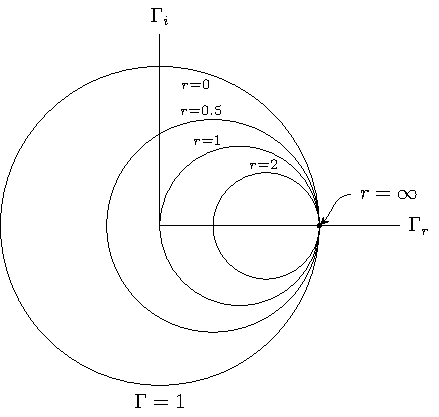
\includegraphics{figTransmissionSmithRealPart}
\caption{کارتیسی محدد کے متغیرات \عددیء{\Gamma_r} اور \عددیء{\Gamma_i} ہیں جبکہ دائرے کا رداس \عددیء{\tfrac{1}{r+1}} ہے۔}
\label{شکل_ترسیلی_سمتھ-نقشہ_الف}
\end{figure}

\begin{figure}
\centering
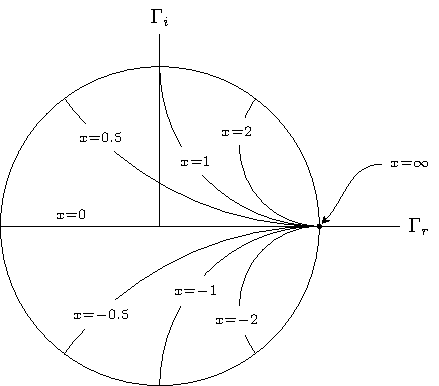
\includegraphics{figTransmissionSmithImaginaryPart}
\caption{کارتیسی محدد پر $\tfrac{1}{x}$ رداس کے دائروں کے وہ حصے دکھائے گئے ہیں جو اکائی دائرے کے اندر پائے جاتے ہیں۔}
\label{شکل_ترسیلی_سمتھ-نقشہ_ب}
\end{figure}
